% Options for packages loaded elsewhere
\PassOptionsToPackage{unicode}{hyperref}
\PassOptionsToPackage{hyphens}{url}
%
\documentclass[
]{article}
\usepackage{amsmath,amssymb}
\usepackage{lmodern}
\usepackage{iftex}
\ifPDFTeX
  \usepackage[T1]{fontenc}
  \usepackage[utf8]{inputenc}
  \usepackage{textcomp} % provide euro and other symbols
\else % if luatex or xetex
  \usepackage{unicode-math}
  \defaultfontfeatures{Scale=MatchLowercase}
  \defaultfontfeatures[\rmfamily]{Ligatures=TeX,Scale=1}
\fi
% Use upquote if available, for straight quotes in verbatim environments
\IfFileExists{upquote.sty}{\usepackage{upquote}}{}
\IfFileExists{microtype.sty}{% use microtype if available
  \usepackage[]{microtype}
  \UseMicrotypeSet[protrusion]{basicmath} % disable protrusion for tt fonts
}{}
\makeatletter
\@ifundefined{KOMAClassName}{% if non-KOMA class
  \IfFileExists{parskip.sty}{%
    \usepackage{parskip}
  }{% else
    \setlength{\parindent}{0pt}
    \setlength{\parskip}{6pt plus 2pt minus 1pt}}
}{% if KOMA class
  \KOMAoptions{parskip=half}}
\makeatother
\usepackage{xcolor}
\usepackage[margin=1in]{geometry}
\usepackage{longtable,booktabs,array}
\usepackage{calc} % for calculating minipage widths
% Correct order of tables after \paragraph or \subparagraph
\usepackage{etoolbox}
\makeatletter
\patchcmd\longtable{\par}{\if@noskipsec\mbox{}\fi\par}{}{}
\makeatother
% Allow footnotes in longtable head/foot
\IfFileExists{footnotehyper.sty}{\usepackage{footnotehyper}}{\usepackage{footnote}}
\makesavenoteenv{longtable}
\usepackage{graphicx}
\makeatletter
\def\maxwidth{\ifdim\Gin@nat@width>\linewidth\linewidth\else\Gin@nat@width\fi}
\def\maxheight{\ifdim\Gin@nat@height>\textheight\textheight\else\Gin@nat@height\fi}
\makeatother
% Scale images if necessary, so that they will not overflow the page
% margins by default, and it is still possible to overwrite the defaults
% using explicit options in \includegraphics[width, height, ...]{}
\setkeys{Gin}{width=\maxwidth,height=\maxheight,keepaspectratio}
% Set default figure placement to htbp
\makeatletter
\def\fps@figure{htbp}
\makeatother
\setlength{\emergencystretch}{3em} % prevent overfull lines
\providecommand{\tightlist}{%
  \setlength{\itemsep}{0pt}\setlength{\parskip}{0pt}}
\setcounter{secnumdepth}{-\maxdimen} % remove section numbering
\usepackage{float}
\let\origfigure\figure
\let\endorigfigure\endfigure
\renewenvironment{figure}[1][2] {
    \expandafter\origfigure\expandafter[H]
} {
    \endorigfigure
}
\usepackage{flafter}
\ifLuaTeX
  \usepackage{selnolig}  % disable illegal ligatures
\fi
\IfFileExists{bookmark.sty}{\usepackage{bookmark}}{\usepackage{hyperref}}
\IfFileExists{xurl.sty}{\usepackage{xurl}}{} % add URL line breaks if available
\urlstyle{same} % disable monospaced font for URLs
\hypersetup{
  pdftitle={Historical algal blooms in the UCFR},
  pdfauthor={Feijo-Lima, Rafael},
  hidelinks,
  pdfcreator={LaTeX via pandoc}}

\title{Historical algal blooms in the UCFR}
\author{Feijo-Lima, Rafael}
\date{2023-06-27}

\begin{document}
\maketitle

\hypertarget{tentative-title}{%
\subsection{Tentative title:}\label{tentative-title}}

``Forecasting (mid summer) algal blooms in a montane river under
multiple stressors: A boosted regression tree approach.''

\hypertarget{background}{%
\subsection{Background}\label{background}}

Algal blooms are everywhere and they are bad. Boooo!

Historic of blooms at the UCFR

Historical changes to Nut inputs. Future directions? (Claire).
Historical monitoring.

Potential changes due to climate change. Freshet has been shown to
influence max growth. Temperature has been shown to influence Cladophora
metabolism. Timing of freshet, temperature and nutrient availability may
have an interplay with secondary cyanobacterial blooms.

Nonlinear relationships and thresholds are not easily captured by
traditional modelling methods, hence Boosted Regression Trees.

One of the strengths of BRTs is the ease to generate predictive models.

\hypertarget{objectives}{%
\subsection{Objectives}\label{objectives}}

Based on the historical datasets, determine the factors predicting algal
blooms in the UCFR.

\begin{itemize}
\tightlist
\item
  Given that future nutrient mitigations are necessary:

  \begin{itemize}
  \tightlist
  \item
    Estimate how previous nutrient reductions may have influenced the
    pervasiveness of algal blooms in the UCFR. (Claire?)
  \item
    Using climatic forecasts, estimate how algal blooms might respond to
    a warming climate under different nutrient scenarios.
  \end{itemize}
\end{itemize}

\hypertarget{methods}{%
\subsection{Methods}\label{methods}}

\hypertarget{historical-datasets}{%
\subsubsection{Historical Datasets:}\label{historical-datasets}}

VNRP data

USGS gauge data

Statistical analyses:

\hypertarget{prior-to-analyses}{%
\subsubsection{Prior to analyses:}\label{prior-to-analyses}}

How much to include? Glms prior to variable selection.

\hypertarget{variable-selection}{%
\subsubsection{Variable Selection}\label{variable-selection}}

Groups:

Temporal selection of nutrient datasets.

Total Nitrogen

Total Phosphorous

Phischem variables from VNRP dataset (Temp, pH).

Temperature

pH

Variables derived from hydrograph.

Q anomaly:

Days since freshet:

\hypertarget{results}{%
\subsection{Results}\label{results}}

\hypertarget{general-patterns-of-main-variables-by-site.-table.}{%
\subsubsection{General patterns of main variables by site.
Table.}\label{general-patterns-of-main-variables-by-site.-table.}}

\begin{longtable}[]{@{}lllllll@{}}
\toprule()
Site & Temp..oC. & pH & TN..mg.l. & TP..mg.l. & pSize & dP \\
\midrule()
\endhead
DL & 13.3 (1.97) & 8.3 (0.14) & 369.9 (82.17) & 25.2 (16.52) & 2 (0.51)
& 66.1 (23.52) \\
GR & 14.7 (3.65) & 8.4 (0.16) & 276.3 (45.64) & 34.7 (16.82) & 2.1 (0.6)
& 66.7 (23.29) \\
BN & 15.3 (2.99) & 8.4 (0.11) & 251.1 (87.55) & 28 (15.76) & 1 (0.29) &
77.1 (30.65) \\
MS & 14.3 (2.46) & 8.2 (0.25) & 183.1 (56.35) & 19 (10.34) & 2.4 (0.5) &
81.5 (25.57) \\
BM & 14.5 (1.92) & 8.3 (0.11) & 202.6 (40.8) & 18.5 (4.62) & 3.8 (0.6) &
82 (27.24) \\
HU & 16.6 (2.75) & 8.3 (0.14) & 213 (46.45) & 16.9 (2.55) & 3.8 (0.6) &
87.4 (20.72) \\
FH & 17.1 (2.4) & 8.4 (0.19) & 152.7 (23.83) & 10.3 (5.09) & 2.2 (0.35)
& 88 (20.13) \\
\bottomrule()
\end{longtable}

Chlorophyll by site (Log)

\begin{figure}

{\centering 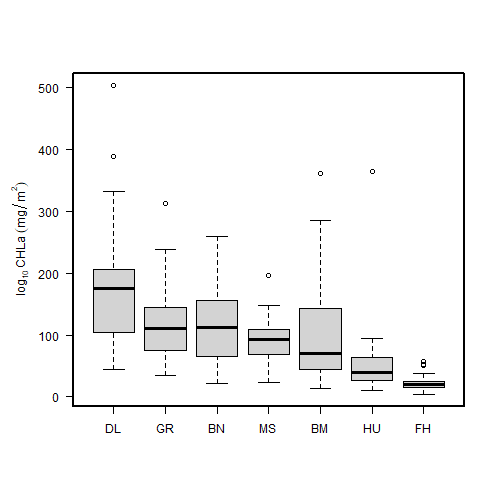
\includegraphics[width=1\linewidth]{Manuscript_files/FIGURES/Chla_Boxplots} 

}

\caption{A caption}\label{fig:unnamed-chunk-1}
\end{figure}

Variance inflation test.

\begin{longtable}[]{@{}rlr@{}}
\toprule()
X & Variables & VIF \\
\midrule()
\endhead
1 & Temperature.oC & 1.252438 \\
2 & pH & 1.135731 \\
3 & TN.ug.l & 1.593165 \\
4 & TP.ug.l & 1.402433 \\
5 & Q.Anomaly & 1.110009 \\
6 & Days.Since.Freshet & 1.107505 \\
\bottomrule()
\end{longtable}

\hypertarget{predicted-vs-observed.-how-to-report-binomial}{%
\subsubsection{Predicted vs observed. How to report
binomial?}\label{predicted-vs-observed.-how-to-report-binomial}}

\begin{figure}
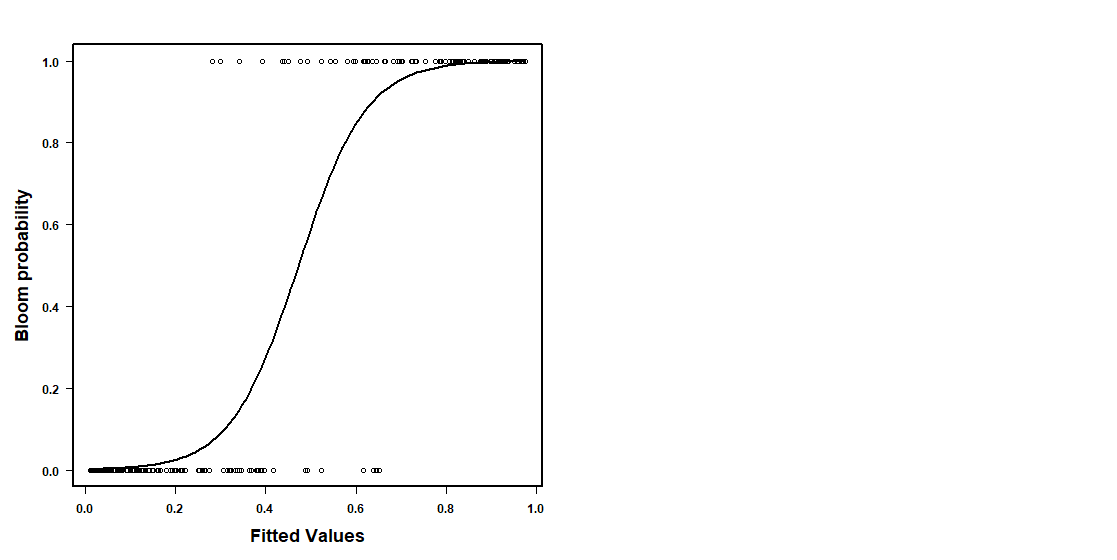
\includegraphics[width=1\linewidth]{Manuscript_files/FIGURES/Predobs} \caption{A caption}\label{fig:unnamed-chunk-2}
\end{figure}

\hypertarget{holdout-deviance-number-of-trees-how-to-report}{%
\subsubsection{Holdout deviance number of trees: How to
report?}\label{holdout-deviance-number-of-trees-how-to-report}}

\begin{figure}
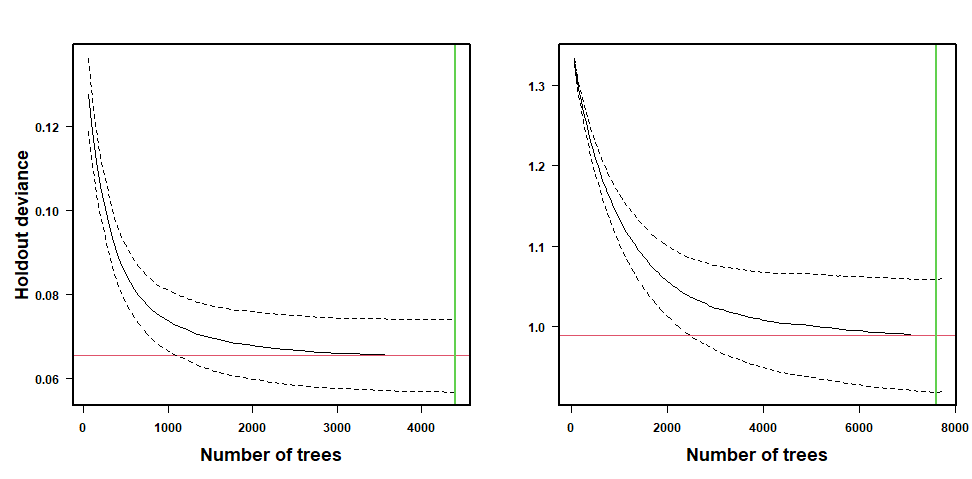
\includegraphics[width=1\linewidth]{Manuscript_files/FIGURES/Holdout_Dev} \caption{A caption}\label{fig:unnamed-chunk-3}
\end{figure}

\hypertarget{partial-dependency-plots.-importance-of-variables.}{%
\subsubsection{Partial dependency plots. Importance of
variables.}\label{partial-dependency-plots.-importance-of-variables.}}

\begin{figure}
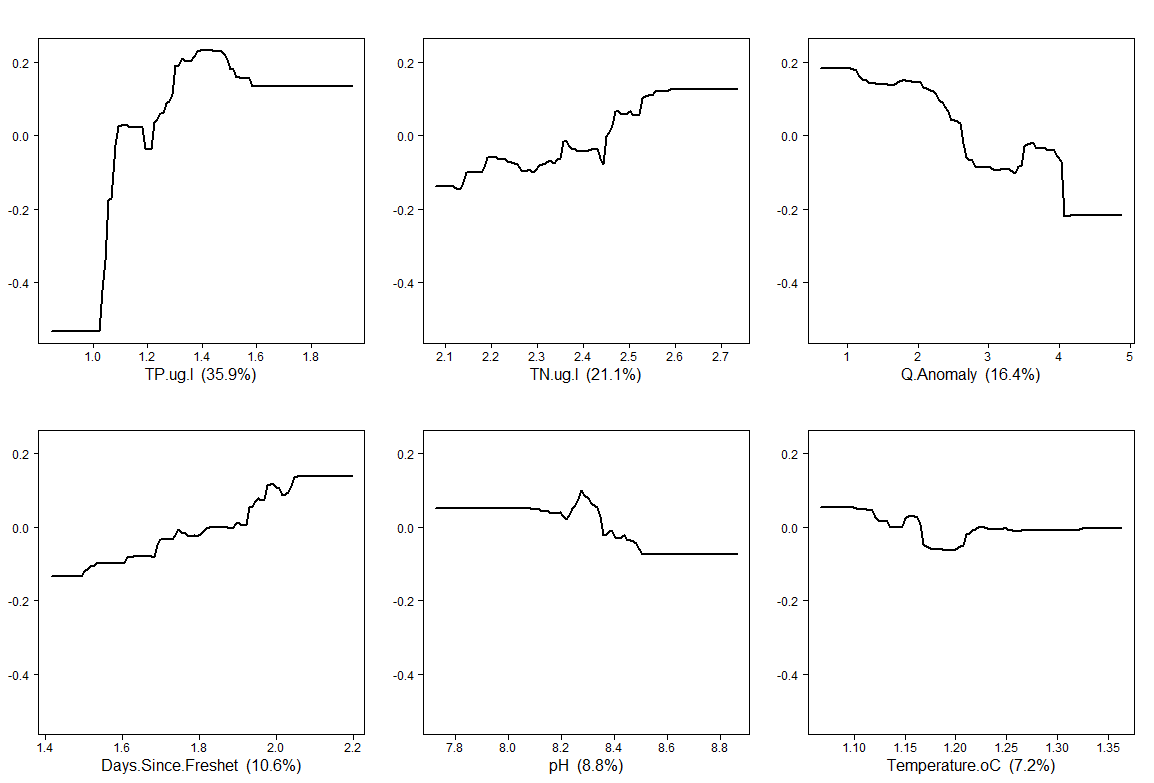
\includegraphics[width=1\linewidth]{Manuscript_files/FIGURES/Part_Dep_SS} \caption{A caption}\label{fig:unnamed-chunk-4}
\end{figure}

\begin{figure}
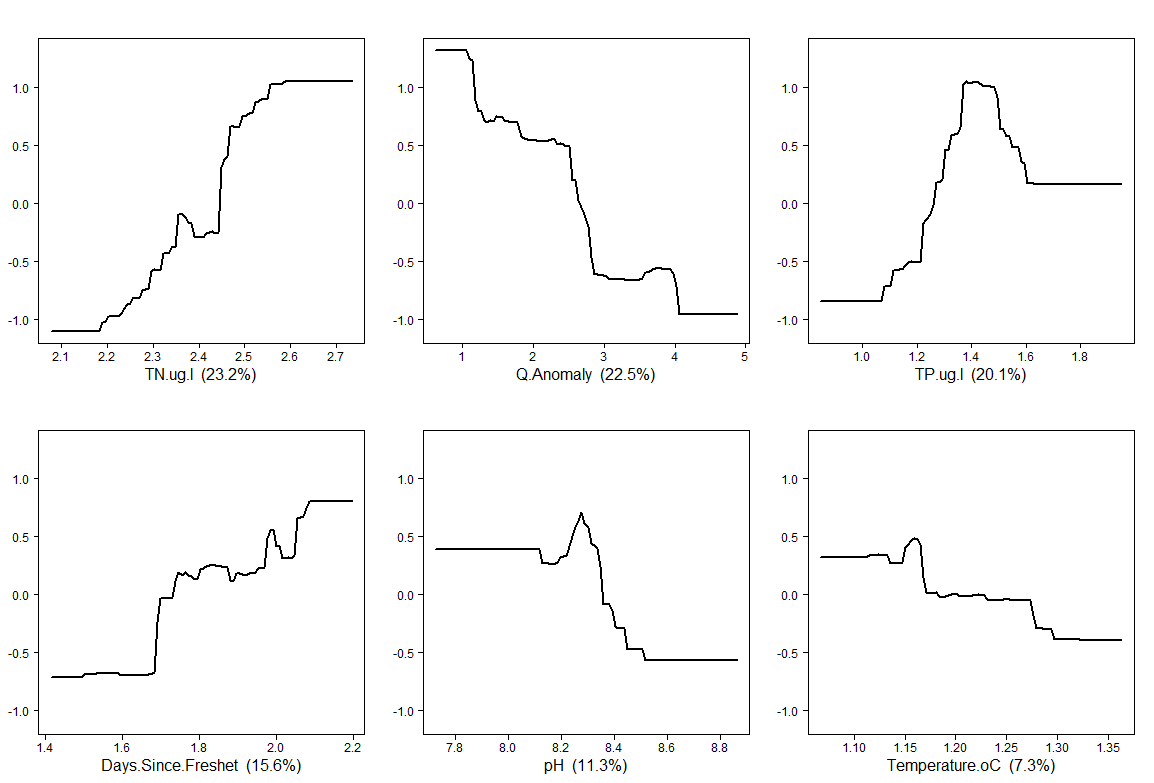
\includegraphics[width=1\linewidth]{Manuscript_files/FIGURES/Part_Dep_BNB} \caption{A caption}\label{fig:unnamed-chunk-5}
\end{figure}

\hypertarget{fitted-values.-appendix}{%
\subsubsection{Fitted Values. Appendix?}\label{fitted-values.-appendix}}

\hypertarget{interaction-plots}{%
\subsubsection{Interaction plots?}\label{interaction-plots}}

\begin{figure}
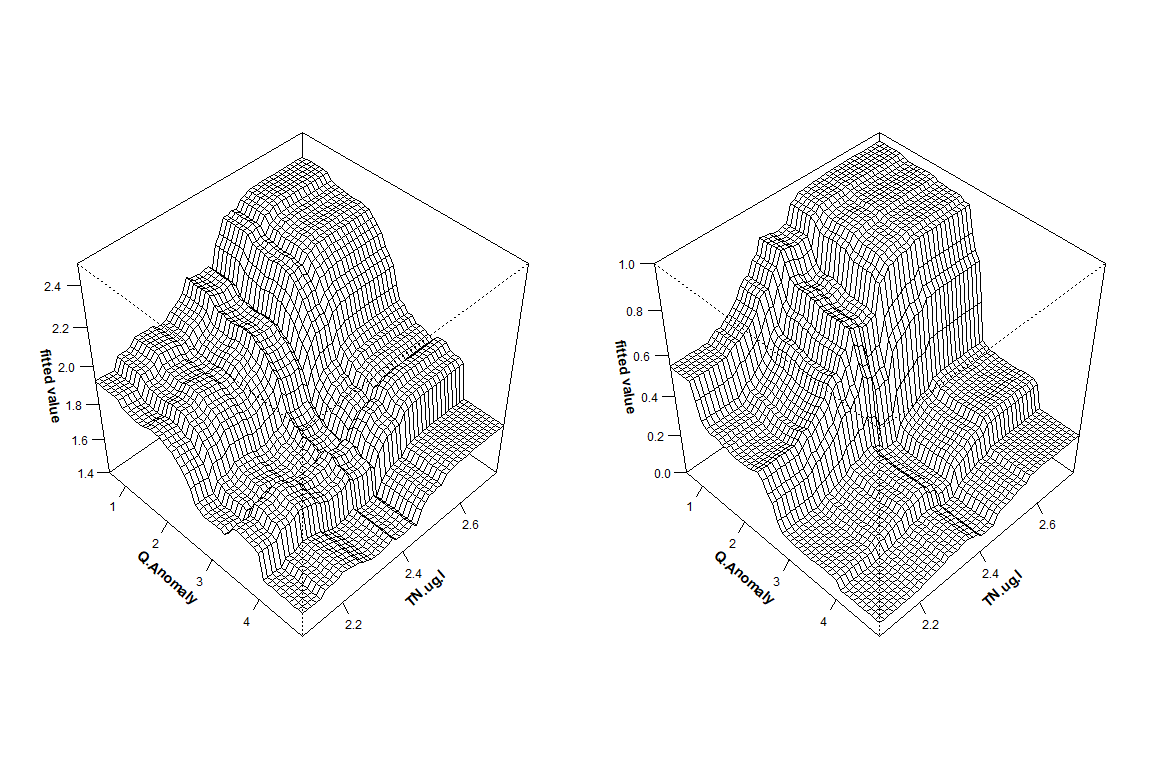
\includegraphics[width=1\linewidth]{Manuscript_files/FIGURES/Interaction_Plots} \caption{A caption}\label{fig:unnamed-chunk-6}
\end{figure}

\hypertarget{discussion}{%
\subsection{Discussion}\label{discussion}}

Performance of boosted regression trees.

Main variables that explained peak biomass.

Implications of future scenarios\ldots{}

\end{document}
